\documentclass[journal]{IEEEtran}
%%\documentclass[journal,onecolumn]{IEEEtran}

\usepackage[utf8]{inputenc}
%%\usepackage{natbib}
\usepackage{multirow}
\usepackage{blindtext}
\usepackage{multicol}
\usepackage{subfigure}
%%\usepackage{graphicx}
\usepackage[portuguese]{babel}
\usepackage{cite}

\ifCLASSINFOpdf
	\usepackage[pdftex]{graphicx}
	\DeclareGraphicsExtensions{.jpg,.jpeg,.png}
\fi

\begin{document}

\title{Dicionário Digital Indígena: Plataforma para catalogação de palavras e expressões das Linguagens Indígenas dos nativos do estado do Tocantins}
\author{
	\IEEEauthorblockN{Lucyano~C.~Martins\IEEEauthorrefmark{1},}
	\IEEEauthorblockN{George~L.~R.~de Brito\IEEEauthorrefmark{1}}\\
	\IEEEauthorblockA{\IEEEauthorrefmark{1}Universidade~Federal~do~Tocantins,~Brasil\\
	lucyano.campos@uft.edu.br}\\
	\IEEEauthorblockA{\IEEEauthorrefmark{1}gbrito@uft.edu.br}
}

\markboth{Pré~projeto~mestrado~,~Vol.~1,~No.~1,~Outubro~2018}{}

\maketitle

\begin{abstract}

O estado do Tocantins conta com várias etnias indígenas nativas, a cidade de Palmas, capital do Tocantins, foi escolhida para sediar Os Jogos Mundiais dos Povos Indígenas no ano de 2015. A preservação e o entendimento sobre as línguas indígenas do Brasil e em especial as nativas Tocantins torna-se essencial para a preservação dos aspectos culturais, no entanto, existe em âmbito nacional e até mesmo mundial a deficiência de ferramentas digitais que possam propiciar o aprendizado ou mesmo entendimento das linguagens indígenas. Essa proposta de projeto contempla o desenvolvimento de uma plataforma para gestão de termos e expressões das linguagens indíginas e seus correspondentes na lingua portuguesa do Brasil, também o desenvolvimento de um aplicativo movél para as plataformas iOS e Android, a fim de proporcionar a sociedade o contato com as culturas nativas do Tocantins.

\end{abstract}

%% Palavras-chave
\begin{IEEEkeywords}
linguagem indígena, dicinonário indígena, cultura indígena
\end{IEEEkeywords}

\section{Introdução}

\IEEEPARstart{A}{tualmente} existe 7 (sete) tribos indígenas vivendo no estado do Tocantins, Brasil, totalizando aproximadamente 10.000 índios, de acordo com informação disponível no Centro de Estudos e Assuntos Indígenas (NEAI) da Universidade Federal do Tocantins \cite{demobile}.

No Brasil são faladas 181 línguas indígenas. Esse número admite pequena margem de erro, para mais ou para menos, em decorrência da imprecisão e, em alguns casos, da distinção entre variedades tão pouco diferenciadas que não dificultam a comunicação entre seus respectivos falantes \cite{silvaterene2013}.

O entendimento da linguagem indígena tem sido objeto de estudo há décadas, sua preservação intensifica o surgimento de pesquisas na área. Com tudo, a deficiência de ferramentas tecnológicas para apoio ainda não amadureceu de maneira a contribuir positivamente e elevar o patamar dos sistemas de entendimento e catalogação para a preservação das línguas nativas brasileiras \cite{abreu2013dicionario}.

De todas as línguas indígenas brasileiras, apenas 13\% possuem uma descrição completa (descrição da gramática, coletânea de textos, dicionário); 38\% possuem descrição avançada (tese de doutorado ou muitos artigos); 29\% possuem descrição incipiente (dissertação de mestrado ou alguns artigos) e 19\% não possuem nada de importância científica. Porém 21\% dessas línguas estão ameaçadas de extinção em curto prazo, sobretudo em decorrência do número reduzido de falantes e da baixa transmissão à nova geração. A situação das demais línguas também é precária, em face do grau de perigo: “O grau de perigo foi subestimado no passado, devido à falta de informações sólidas sobre as línguas em regiões remotas e devido também à confusão entre o número de falantes e ao tamanho da população dos grupos indígenas” \cite{moore2008}.

O Desenvolvimento de uma dicionário eletrônico para catalogação dos termos e expressões indígneas, poderá contribuir com a preservação da cultura nativa. Também dará visibilidade para Universidade Federal do Tocantins, como sendo sua mantenedora, provendo a todos pequisadores da área, fazendo assim que o banco de dados de termos possa crescer conforme a colaboração.

A cultura da língua portuguesa, tanto oral quanto escrita, é para a população indígena no Brasil um grande desafo. Essa língua é economicamente forte, politicamente também \cite{eduardo2018}.

\section{Objetivos Gerais}

Esta proposta de pesquisa tem por objetivo desenvolver uma plataforma para catalogação de termos e expressões indígenas das tribos nativas do Tocantins. Disponibilizando o mesmo em um sistema multiplataforma ({\it API \footnote{{\it API - Application Programming Interface} que significa em tradução para o português Interface de Programação de Aplicativos.}, web, mobile}).

A finalidade da disponibilização da {\it API} é a posibilidade de integração com outras pesquisas nesse campo, tornando a {\bf Universidade Federal do Tocantins} pioneira nesse aspecto. Também destina-se a possibidade do desenvolvimento de mais ferramentas para contato final com a sociedade, exemplos: aplicativos {\it mobile}, {\it web} e ferramentas de terceiros.

O desenvolvimento e entrada do aplicativo para plataformas {\it mobile} iOS e Android possibilitará o maior contato da sociedade em geral com o objeto desse trabalho, que é a catalogação dos termos indígenas. 

\section{Objetivos Específicos}

\begin{itemize}
    \item Estudo das linguagens indígenas iniciais: tronco linguístico Macro-Jê\footnote{Tronco lingüístico comum dos povos: Karajá, Javaé e Xambioá}, Apinayé e Kraô;
    \item Criação da infraestrutura necessário para os sistemas: servidor; banco de dados e CDN\footnote{CDN é abreviação de {\it Content Delivery Network} ou Rede de Distribuição de Conteúdo. };
    \item Desenvolvimento da camada {\it Web} para gerenciamento de conteúdo CMS\footnote{{\it Content Management System}, Sistema Gerenciador de Conteúdo};
    \item Desenvolvimento da {\it API} de integração;
    \item Desenvolvimento dos aplicativos {\it mobile: iOS};
    \item Desenvolvimento dos aplicativos {\it mobile: Android};
    \item Desenvolvimento {\it Hotsite} do Dicionário Eletrônico Indígena;
    \item Divulgação da plataforma;
\end{itemize}

\section{Delimitação}

A abrangência do estudo deste trabalho é destinado especificamente as demandas regionais do estudo das linguas das tribos nativas do Tocantins. Percebendo o seu valor cultural e importância da manutenção de sua existência, e observando o contexto regial que a Universidade Federal do Tocantins está inserida.

\section{Justificativa}

O desenvolvimento do objeto dessa pesquisa, busca agregar fatores recorrentes na sociedade do estado do Tocantins. Um deles diz respeito ao contato da população indígena com os grandes centros urbanos, o que traz desconforto pela falta de comunicação em suas línguas nativas, também o conhecimento e contato da sociedade em geral com a cultura indígena.

A consolidação desse estudo, possibilitará o catalogamente e mesmo disponibilização do estudo em um cenário maior, trará ao trabalho um valor cultural substâncial, podendo transformar o objeto dessa pesquisa em padrão que pode ser adotado nacionalmente, e posteriormente apresentado no contexto internacional, a depender de sua relevância e aceitação.

\section{Questões Problemas}

Já existe em âmbito nacional diversas pesquisas para mapeamento das línguas indígenas com seu correspondente na língua portuguesa, trabalhos que tiveram como objetivo a criação de dicionários indígenas, exemplos: Dicionário Ilustrado Tupi Guarani, Dicionário Indígena - Museu do Índio, Estudo Lexicográfico da Língua Terena - Desine Silva, 2013, dentre outros.

Este trabalho destina-se a apoiar-se nessas pesquisas, no intuito de catalogar resultados já antes pesquisados, validados e apresentados.
\\
\\
{\bf Questões síntese do problema}

\begin{itemize}
    \item Facilitar o acesso a linguagem indígena a população urbana;
    \item Preservar os estudos das linguagens indígena;
    \item Criar um repositório para estudos e preservação das linguagens indígenas;
    \item Tornar a UFT mantenedora dessa ferramenta;
\end{itemize}

\section{Materiais e Métodos}

O método de trabalho para condução desta pesquisa é composto por pesquisa bibliográfica e pesquisa técnica. Com o objetivo de adquirir competências para a condução da pesquisa técnica, a pesquisa bibliográfica abordará os seguintes assuntos, com as respectivas finalidades:
\\
\begin{itemize}
    \item Entendimento das linguagens indígenas;
    \item Modelagem do sistema e {\it frameworks} necessários;
    \item Pesquisa técnica: Principais plataformas para desenvolvimento web e mobile, técnicas de distribuição de conteúdo por meio de {\it API}.
\end{itemize}

\section{Referencial Teórico}

Como base para essa pesquisa o trabalho de conclusão e curso com o título {\it “Desenvolvimento de uma Plataforma Online de tradução da linguagem indígena Xerente para linguagem Portuguesa”}, do autor {\bf Alain Neves Lima} do ano de 2014 da Universidade Federal do Tocantins (UFT), contém pesquisa realizada no campo da tradução indígena e como produto final o aplicativo {\it mobile  Traduzíndio}.

%O livro do pesquisador {\bf Aryon Dalligna Rodrigues} com o título {\it "Línguas brasileiras: pra o conhecimento das línguas indígenas"} do %ano de 2002 contém estudos relevantes acerca da histórias e entendimentos das linguagens indígenas brasileiras. 

Quem queira desenvolver seus próprios estudos sobre uma língua determinada ou sobre um conjunto de línguas deve procurar as obras que tratam especialmente dessas línguas e dos povos que as falam \cite{rodrigues2002}.

Para apoio no entendimento da tradução indígena Xerente o {\it “Dicionário Escolar: Xerente - Português; Português – Xerente”}, dos autores: {\bf Wanda Braidotti Krieger e Guenther Carlos Krieger} do ano de 1994.

\section{Cronograma de Atividades}

A listagem das atividades necessárias ao desenvolvimento do projeto de pesquisa e as respectivas durações estimadas (em trimestres) compõem o cronograma apresentado no Quadro 1. Embora a abrangência temporal das atividades no cronograma seja mostrada trimestralmente, estima-se que a duração de algumas atividades listadas seja inferior a três meses.

\begin{table}[!ht]
	\centering
	\caption{Cronograma de Atividades para desenvolvimento deste trabalho}
	\begin{tabular}{|l|c|c|c|c|c|c|c|c|} \hline
	 \multirow{2}{*}{}& \multicolumn{2}{c|}{{\bf2018}}& \multicolumn{4}{c|}{{\bf2019}}& \multicolumn{2}{c|}{{\bf2020}}
	 \\ \cline{2-9} 
                       				              &  3  &  4  &  1  &  2  &  3  &  4  &  1  &  2 \\ \hline
		\scriptsize{Pesquisa bibliográfica} 	  &  X  &  X  &     &     &     &     &     &    \\ \hline
		\scriptsize{Pesquisa técnica}	          &     &  X  &  X  &     &     &     &     &    \\ \hline
		\scriptsize{Estudo línguas indígenas}	  &     &  X  &  X  &     &     &     &     &    \\ \hline
		\scriptsize{Modelagem do Sistema}	      &     &  X  &  X  &     &     &     &     &    \\ \hline
	    \scriptsize{Criação infraestrutura}       &     &     &     &  X  &  X  &     &     &    \\ \hline
	    \scriptsize{Desenvolvimento da Plataforma}&     &     &     &  X  &  X  &     &     &    \\ \hline
	    \scriptsize{Implantação da Plataforma}    &     &     &     &     &     &  X  &     &    \\ \hline
	    \scriptsize{Elaboração de artigos}        &     &     &  X  &  X  &  X  &  X  &     &    \\ \hline
	    \scriptsize{Defesa da dissertação}        &     &     &     &     &  X  &  X  &  X  &  X \\ \hline
	\end{tabular}
	\label{t_cronograma}
\end{table}

%%\begin{table}[!ht]
%%	\centering
%%	\caption{Cronograma de Atividades para desenvolvimento deste trabalho}
%%	\begin{tabular}{|l l|c|c|c|c|c|c|c|c|} \hline
%%		\multirow{2}{*}{} & \multirow{2}{*}{} & \multicolumn{2}{c|}{{\bf2018}} & \multicolumn{4}{c|}{{\bf2019}}& \multicolumn{2}{c|}{{\bf2020}}   \\ \cline{3-10} 
%%            &   				                                        &  3  &  4  &  1  &  2  &  3  &  4  &  1  &  2 \\ \hline
%%		\scriptsize{1.}&\scriptsize{Pesquisa bibliográfica} 	                        &  X  &  X  &     &     &     &     &     &    \\ \hline
%%		\scriptsize{2.}&\scriptsize{Pesquisa técnica}	                                &     &  X  &  X  &     &     &     &     &    \\ \hline
%%		\scriptsize{3.}&\scriptsize{Estudo línguas indígenas do Tocantins}	            &     &  X  &  X  &     &     &     &     &    \\ \hline
%%		\scriptsize{4.}&\scriptsize{Modelagem do Sistema}	                            &     &     &  X  &  X  &     &     &     &    \\ \hline
%%	    \scriptsize{5.}&\scriptsize{Criação infraestrutura}                             &     &     &     &  X  &  X  &     &     &    \\ \hline
%%	    \scriptsize{6.}&\scriptsize{Desenvolvimento da Plataforma}                      &     &     &     &  X  &  X  &     &     &    \\ \hline
%%	    \scriptsize{7.}&\scriptsize{Implantação da Plataforma}                          &     &     &     &     &     &  X  &     &    \\ \hline
%%	    \scriptsize{8.}&\scriptsize{Elaboração de artigos científicos para revistas}    &     &     &  X  &  X  &  X  &  X  &     &    \\ \hline
%%	    \scriptsize{9.}&\scriptsize{Elaboração e defesa da dissertação}                 &     &     &     &     &  X  &  X  &  X  &  X \\ \hline
%%	\end{tabular}
%%	\label{t_cronograma}
%%\end{table}

\section{Resultados Esperados}

O entrega final desse trabalho tem como objetivo os seguintes itens:

\begin{itemize}
    \item Plataforma para gerenciamento da catalogação dos termos e expressões indígenas;
    \item Hotsite apresentando o projeto e também disponibilizando o acesso ao dicinário;
    \item Aplicativo iOS Dicionário de Linguagens Indígenas;
    \item Aplicativo Android Dicionário de Linguagens Indígenas;
\end{itemize}

\section{Escopo do Projeto}

O projeto está divido em 4 gradnes entregas: Aprendizado Lianguagem Indígena, Modelagem do Sistema, Desenvolvimento (Implementação) e Entrega do Produto Final.

\begin{table}[!ht] 
	\centering
	\caption{Fases do Projeto.}
		\begin{tabular}{l|c}
			\hline
				{\bf Fase} & {\bf \%}\\
			\hline
				Aprendizado     & 20\% \\
				Modelagem       & 30\% \\
				Desenvolvimento & 40\% \\
				Entrega         & 10\% \\
			\hline
				{\bf TOTAL} & {\bf 100\%}\\
			\hline
		\end{tabular}
	\label{t:modelo}
\end{table}

\begin{figure}[!ht]
	\centering
	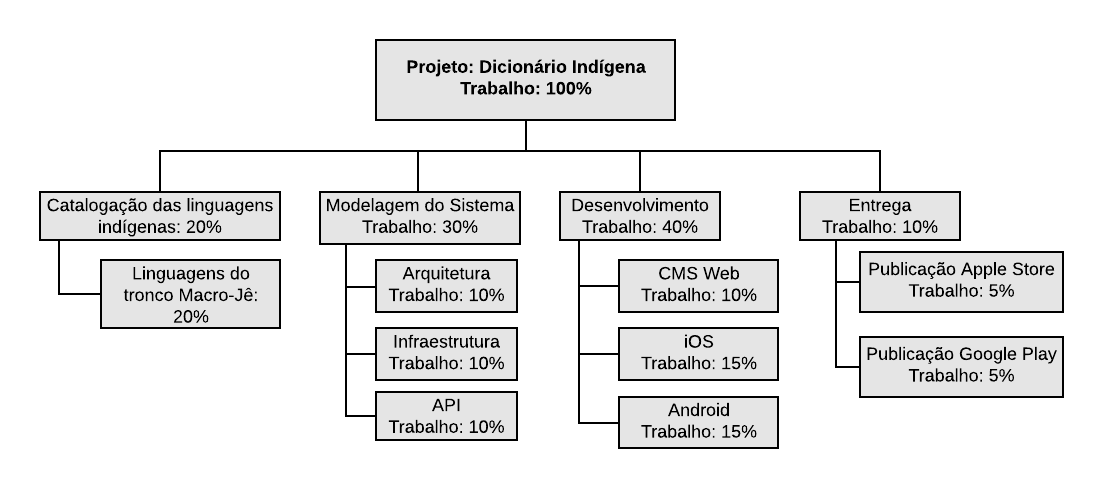
\includegraphics[scale=0.55]{eap.png}
	\caption{Diagrama de Estrutura Analítica do Projeto}
	\label{f:latex12c}
\end{figure}

\bibliographystyle{IEEEtran}
\bibliography{referencias}

\begin{IEEEbiography}
[{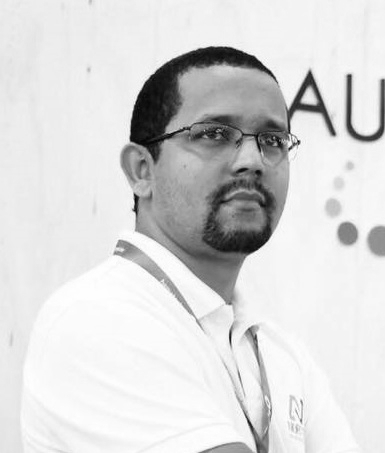
\includegraphics[width=1in,height=1.25in,clip,keepaspectratio]{lucyano.jpg}}]{Lucyano Campos Martins}
Aluno do programa de Mestrado Profissional em Modelagem Computacional da Universidade Federal do Tocantins, Especialista em Gestão da Tecnologia da Informação pela Faculdade Católica do Tocantins, Palmas-TO, conclusão 2010. Bacharel em Sistemas de Informação pelo Centro Universitário ITPAC (UNITPAC), Araguaína-TO, conclusão 2009. Técnico em Informática com ênfase em programação pela Escola Agrotécnica Federal de Inconfidentes-MG, conclusão 2003.
\end{IEEEbiography}

\begin{IEEEbiography}
[{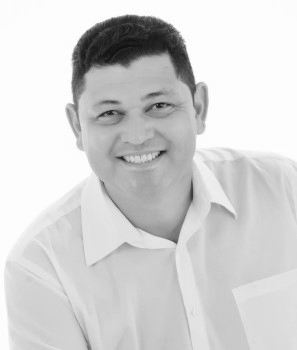
\includegraphics[width=1in,height=1.25in,clip,keepaspectratio]{george.jpg}}]{George Lauro Ribeiro de Brito}
Possui Graduação em Engenharia Elétrica pela Universidade Federal de Mato Grosso (2000), Especialização em Gestão Pública pela Universidade Federal do Tocantins (2013), Mestrado em Engenharia Elétrica pela Universidade de São Paulo (2003) e Doutorado em Engenharia Elétrica pela Universidade de Brasília (2009); é Professor Associado da Fundação Universidade Federal do Tocantins - UFT. Tem experiência na área de Engenharia Elétrica, com ênfase em Sistemas Elétricos de Potência.
\end{IEEEbiography}

\end{document}
